\chapter{Systemy informatyczne w logistyce}
\label{c3:c3}

\section{Informatyka jako multidyscyplinarna dziedzina wiedzy}
	Informatyka jest rozległą dziedziną nie tyle wiedzy, co zbioru zasad oraz reguł postępowania.
	Z tego powodu należy ją rozpatrywać jako:
	\begin{itemize}
		\item samodzielną dyscyplinę naukową,
		\item narzędzie wykorzystywane przez inne nauki,
		\item gałąź techniki,
		\item przemysł wytwarzający sprzęt i oprogramowanie.
	\end{itemize}	 

	Informatyka bada i jednocześnie zajmuje się definiowaniem przepływu informacji i sposobów jej przetwarzania. 
	Można powiedzieć, że jako dyscyplina naukowa informatyka 
	jako pierwsza z nauk zaczęła badać \textbf{prawa rządzące przetwarzaniem informacji}, czyli notabene
	tak zwanej \emph{wiedzy wtórnej}. Jednocześnie informatyka stworzyła wciąż rosnący i mający 
	ogromy potencjał rynek przemysłu komputerowego, który z jednej strony definiuje, a który 
	z drugiej strony wymusza rozwój nauki, która go stworzyła \cite{it_definition}.\\
	
	W czasach społeczeństwa informacyjnego, przemysłu, życia osobistego zdominowanego przez potęgę informacji, informatyka
	przestała być tylko nauką, a stała się narzędziem. Narzędzie to używane jest praktycznie wszędzie
	we wszystkich swoich odmianach i mutacjach. Nie można wyobrazić sobie dzisiaj małego osiedla sklepowego bez
	kasy fiskalnej, do której przecież trzeba było napisać stosowne oprogramowanie sterujące i stworzyć
	elementy fizycznej struktury. Ciężko będzie znaleźć kogoś, kto nie korzysta dzisiaj z dobrodziejstw poczty
	elektronicznej, czy też ciągle rosnącego segmentu usług społecznościowych. Informatyka obecna jest we
	wszystkich aspektach życia, nawet jeśli nie zdajemy sobie z tego sprawy.
	
\section{Znaczenie informatyki w świecie logistyków}
	\begin{quote}
		\textit{
			``Największym zagrożeniem dla dzisiejszej firmy jest niezdolność do dostrzegania związku
			między dzisiejszą fikcją i jutrzejszą rzeczywistością
			\footnote{prof. Piotr Płoszajski, sprawozdanie z III Forum Praktykantów Logistyki.\\
			\url{http://spedycje.pl/logistyka/pod_znakiem_logistyka/12003/informatyzacja_logistyki.html}}''.
		}
	\end{quote}

	Współcześnie realizowana logistyka opiera się na technologiach informatycznych i w swojej rozbudowanej
	formie, w konieczności objęcia swoim zasięgiem wielu różnorodnych problemów, byłaby po prostu instrumentem
	niewygodnym. Dzięki wsparciu nauk informatycznych, logistyka od kilkunastu, jeśli nie kilkudziesięciu lat,
	istnieje jako samodzielny byt, dawno oderwany od swojego stereotypowego kojarzenia z transportem. Głównym
	powodem takiego stanu rzeczy są \textbf{zintegrowane systemy informatyczne}, wspierające efektywne zarządzanie
	przedsiębiorstwami zarówno globalnymi, jak i lokalnymi. To co łączy wszystkie systemy informatyczne to
	z pewnością zasada, według której system powinien wspierać procesy zachodzące w organizacji, od najwcześniejszego
	możliwego momentu, do chwili, kiedy gotowy produkt / usługa zostanie dostarczona do klienta. \\
	
	Procesy logistyczne, produkcyjne, dystrybucji czy też magazynowanie znacznie różnią się od tych, jakie istniały
	w czasach wielkich rewolucji przemysłowych. Liniowe łańcuchy dostaw zastąpione zostały przez złożone siatki dostawców i odbiorców,
	działających już nie w skali powiatu lub województwa, ale w skali całego kontynentu czy też świata. Dawno
	już zniknęły proste sposoby ewidencji towarów opartych na systemie kartka papieru i długopis. Ich miejsce zajęły
	kompleksowe bazy danych wraz z równie rozbudowanymi interfejsami użytkownika. Te i inne podobne zmiany można
	uznać za podwaliny czy też synonim znaczenia informatyki dla logistyki współczesnej. \\ 
	
	Informatyka przychodząc ze swoimi możliwościami przetwarzania danych w sposób nie tyle atomowy, co uwzględniający
	skomplikowane powiązania między informacjami, dała logistykom oręż potrzebny do modelowania 
	fizycznych związków występujących między przedsiębiorcami oraz klientami, czy też utrzymania i prowadzenia
	ewidencji wydań oraz przyjęć czy też nawet zwrotów i ostatecznie wsparcia gospodarki materiałowej \cite{IDL}.
	
\pagebreak
\section{Pojęcie systemu informatycznego}	
	Współcześnie systemy logistyczne charakteryzują się złożonością zarówno wewnętrznych oraz zewnętrznych
	procesów przepływu zasobów materiałowych, finansowych i informacyjnych. są jednym z najważniejszych filarów
	współczesnej logistyki.
	\begin{figure}[h]
		\centering
		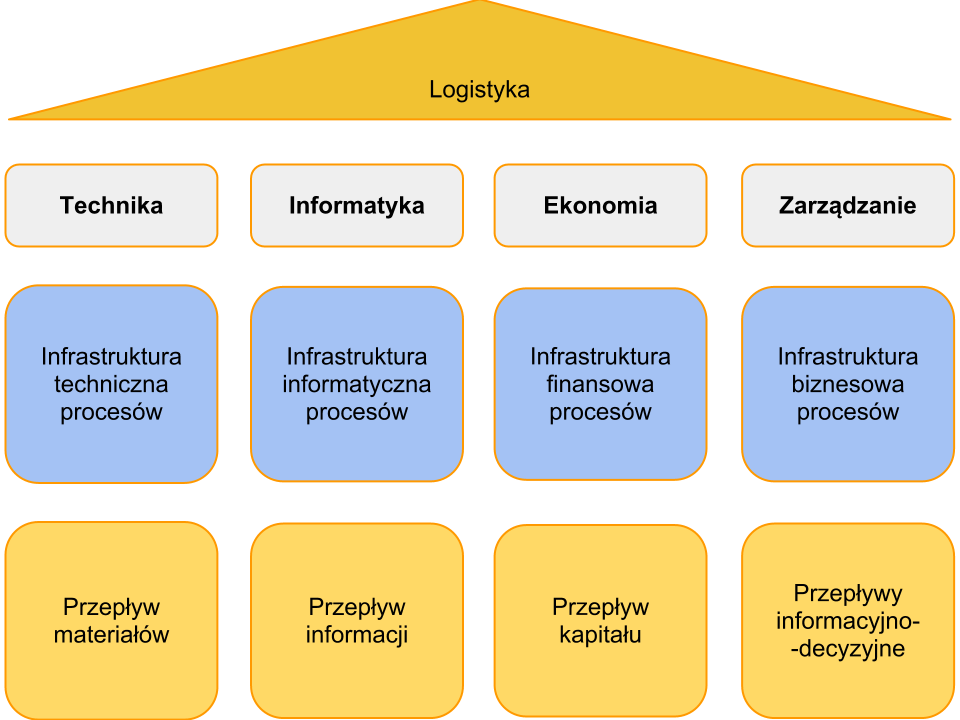
\includegraphics[width=0.95\textwidth]{images/filary_logistyki}
		\caption[Główne filary logistyki]{
			Główne filary logistyki\\
			źródło: \cite{logistyka_w_przedsiebiorstwie}
		}
	\end{figure}
	Żyjemy dzisiaj coraz szybciej i to właśnie szybkość oraz globalizacja rynków i konkurencji
	implikujących efektywność przetwarzania informacji, wymusiły wykorzystanie odpowiednich
	systemów informatycznych, umożliwiających obieg, przetwarzanie, udostępnienia, magazynowanie
	i archiwizowanie informacji, istotnych dla systemu lub jego użytkownika.  	
	
	\subsection{Czym jest system informatyczny ?}
		\begin{figure}[H]
			\centering
			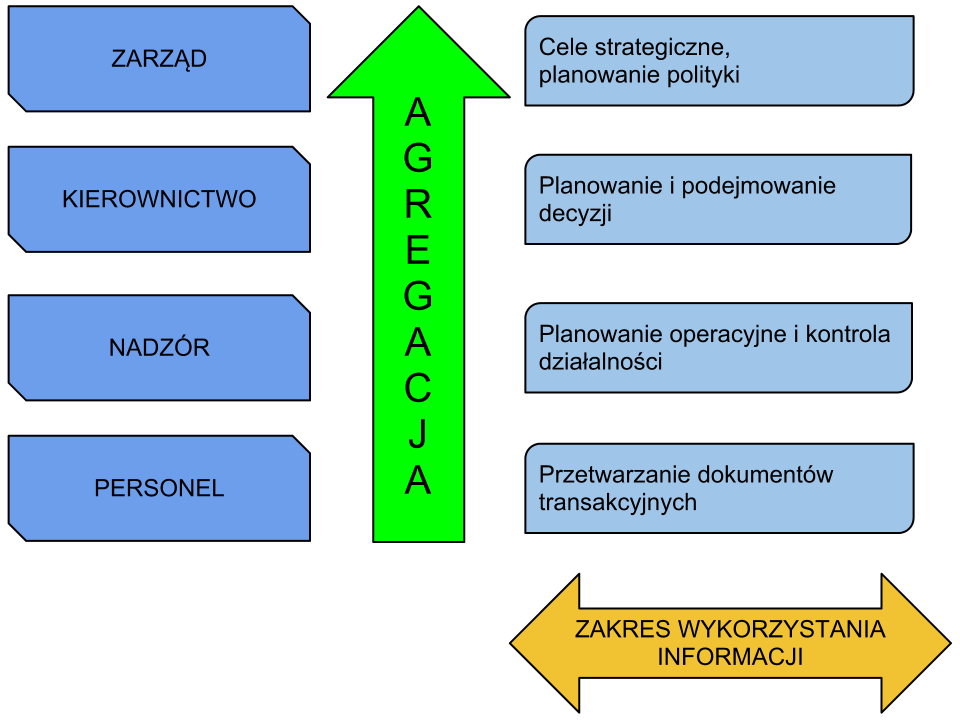
\includegraphics[width=0.95\textwidth]{images/poziomy_agregacji_informacji}
			\caption[Poziomy agregacji informacji w systemie informatycznym]{
				Poziomy agregacji informacji\\ 
				źródło: \cite{IDL}
			}
			\label{c3:information_level_figure}
		\end{figure}
		System informatyczny jest kompleksowym bytem, którego głównym zadaniem 
		jest udos\-tępnienia narzędzi do efektywnego przetwarzania informacji. 
		Na system informatyczny składają się następujące powiązane ze sobą elementy:
		\begin{itemize}
			\item \textbf{sprzęt informatyczny} - wszelkie urządzenia służące
			do przechowywania danych, komunikacji między modułami systemu, zestawy urządzeń
			peryferyjnych umożliwiających człowiekowi pracę z systemem lub też wszelkie urządzenia
			automatycznie kontrolowane przez system informatyczny jak np. magazyny wysokiego składu;
			\item \textbf{oprogramowanie} - zainstalowanego na komputerach z przeznaczeniem realizacji
			wyznaczonych zadań,
			\item \textbf{zasoby ludzkie} - programiści oraz osoby obsługujące komputery,
			\item \textbf{elementów organizacyjnych} - procedur korzystania z systemu informatycznego,
			\item \textbf{baz wiedzy} \cite{logistyka_w_przedsiebiorstwie}.
		\end{itemize}
		
		\paragraph{System informatyczny, czy system informacyjny ?}
		System informatyczny można traktować jako narzędzia udostępniające użytkownikom 
		obszerną funkcjonalność, pozwalającą na przetwarzanie różnych kolekcji danych.
		To właśnie dane, zapisane w bazach danych, będące niepodzielnymi faktami, są 
		spoiwem dla systemu informacyjnego. Informacja jest rezultatem działania
		narzędzi wbudowanych w systemy informatyczne i wynikiem przetwo\-rzenia danych 
		atomowych z jednej postaci w inną. Uzyskujemy w ten sposób wiedzę wtórną, której można 
		użyć na różnych szczeblach zarządzania przedsiębiorstwem (rys: \ref{c3:information_level_figure}). \\
		
		Główny strumień informacji przebiega w większości przedsiębiorstw zgodnie z kierunkiem: 
		\textbf{od zaopatrzenia w materiały i surowce, poprzez ich magazynowanie, następnie przetwo\-rzenie 
		w produkty, składowanie towarów i sprzedaż}. Informacje te, które możemy uznać za krytyczne
		i niezbędne, wspomagane są przez informacje spływające w czasie rzeczywistym z innych działów. 
		W obszarze strumienia informacji występują zarówno miejsca powstania kosztów, jak i zysków.  \\
		
		Systemy informatyczne stosowane do wspomagania logistyki stanowią więc narzędzie, które
		ułatwia pozyskiwanie użytecznych informacji oraz ich analizę dla potrzeb różnego rodzaju. 
		Pojęcie systemu informacyjnego nie funkcjonuje jako określenie faktycznego systemu, działającego
		w przedsiębiorstwach. Jest ona opisem wszystkich tych danych, które można uzyskać, korzystając
		z narzędzi analitycznych, wyszukiwanie itp. dostarczonych wraz z systemem informatycznym.
		
	\subsection{Rodzaje systemów informatycznych w logistyce}
		\begin{center}
			\begin{longtable}{| l | l | l |}
					\caption[Kategorie systemów informatycznych w logistyce]{
						Kategorie systemów informatycznych w logistyce\\
						źródło: opracowanie własne na podstawie \cite{IDL}
					}\\
					\hline
						\multicolumn{1}{|c|}{\textbf{Skrót}}	& 
						\multicolumn{1}{|c|}{\textbf{Nazwa angielska}}	&
						\multicolumn{1}{|c|}{\textbf{Nazwa polska}}	\\
					\hline
					\endfirsthead
					
					\multicolumn{3}{c}%
					{{\bfseries \tablename\ \thetable{} -- kontynuacja...}} \\
					\hline 
						\multicolumn{1}{|c|}{\textbf{Skrót}}	& 
						\multicolumn{1}{|c|}{\textbf{Nazwa angielska}}	&
						\multicolumn{1}{|c|}{\textbf{Nazwa polska}}	\\
					\hline 
					\endhead	
					
					\hline
						\multicolumn{3}{|r|}{{Następna strona...}} \\ \hline
					\endfoot
	
					\hline \hline
					\endlastfoot			
					
					MIS					& Management Information Systems 				& Systemy informacyjne zarządzania	\\
					\hline
					DSS					& Decision Support Systems						& Systemy wspomagania decyzji		\\
					\hline
					MSS					& Management Support Systems					& Systemy wspomagania zarządzania	\\
					\hline	
					EIS					& Executive Information Systems					& Systemy informacyjne kierownictwa	\\
					\hline	
					ESS					& Executive Support Systems						& Systemy wspomagające kierownictwo	\\
					\hline	
					MSS					& Management Support Systems					& Systemy wspomagania zarządzania	\\
					\hline	
					EX					& Expert Systems								& Systemy eksperckie	\\
					\hline	
					KBS					& Knowledge-Based Systems						& Systemy oparte na bazach wiedzy	\\
					\hline	
					TPS					& Transaction Processing Systems				& Systemy transakcyjne	\\
					\hline
			\end{longtable}
		\end{center}		
		
		W kontekście omawianych systemów informatycznych do najczęściej wykorzystywanych zalicza się systemy typu
		\textbf{CAD, SCM oraz WMS}. Systemy \textbf{ERP} zalicza się do klasy wspierającej planowanie, dzięki 
		wbudowanym algorytmom z rodziny metod typu \textbf{MRPI} oraz \textbf{MRPII}.
		
		\begin{center}
			\begin{longtable}{| l | l | p{9.5cm} |}
					\caption[Wybrane kategorie systemów wspomagających logistykę]{
						Wybrane kategorie systemów informatycznych wspomagających logistykę,\\
						źródło: opracowanie własne na podstawie \cite{IDL}
					}\\
					\hline
						\multicolumn{1}{|c|}{\textbf{Skrót}}	& 
						\multicolumn{1}{|c|}{\textbf{System}}	&
						\multicolumn{1}{|c|}{\textbf{Funkcja}}	\\
					\hline
					\endfirsthead
					
					\multicolumn{3}{c}%
					{{\bfseries \tablename\ \thetable{} -- kontynuacja...}} \\
					\hline 
						\multicolumn{1}{|c|}{\textbf{Skrót}}	& 
						\multicolumn{1}{|c|}{\textbf{System}}	&
						\multicolumn{1}{|c|}{\textbf{Funkcja}}	\\
					\hline 
					\endhead	
					
					\hline
						\multicolumn{3}{|r|}{{Następna strona...}} \\ \hline
					\endfoot
	
					\hline \hline
					\endlastfoot			
					
					FK					& Finansowo księgowy 				& Systemy finansowo-księgowe
					zostały stworzone z myślą o optymalizacji procesów finansowych zachodzących
					wewnątrz przedsiębiorstw. Z tego powodu dostarczają one funkcji, pozwalających
					na śledzenie środków trwałych, amortyzacji, regulowania zobowiązań wobec partnerów
					handlowych. Niezaprzeczalną korzyścią posiadania takiego rozwiązania jest możliwość
					monitorowania przepływów pieniężnych, utrzymania pełnej i zwartej historii finansowej
					czy też generowanie raportów na potrzeby decyzji na szczeblach kierowniczych lub
					strategicznych \cite{fk_system}. 	\\
					\hline
					CAD					& Computer Aided Design				& Aplikacje komputerowe
					stworzone z myślą o wspomaganiu projektowania technologicznego-konstrukcyjnego. System
					CAD pozwalają na stworzeniu dowolnego rodzaju modelu. Oprogramowanie tej klasy 
					został pozwala na podniesienie produktywności inżynierów oraz łączenie ze sobą
					wielu modeli w jedną całość. 		\\
					\hline
					ERP					& Enterprise Resource Planning		& Systemy Planowania Zasobów 
					Przedsiębiorstwa należą do grupy zintegrowanych systemów informatycznych, co oznacza
					że składają się z wielu modułów, które współpracując ze sobą, dostarczają
					kompleksowej wiedzy o kondycji, aktualnym stanie przedsiębiorstwa. Wszystkie funkcje, 
					które znaleźć można oczywiście znaleźć w pojedynczych systemach, zostały umieszczone
					w jednym miejscu. Dzięki temu są one uniwersalne i możliwe do wykorzystanie nie tylko
					w firmach o profilu produkcyjnym, ale również i dystrybucyjnym. Główną ich zaletą jest
					zwiększona kontrola i efektywność procesów planowania zamówień oraz sprzedaży, kontrola
					procesów biznesowych w kontekście organizacji oraz automatyzacja czynności, do tej pory
					wykonywanych przez człowieka \cite{erp_system}.\\
					\hline	
					SCM					& Supply Chain Management			& Systemy Zarządzania Łańcuchem
					Dostaw są wykorzystywane do koordynacji kompleksowych procesów obsługujących 
					przepływy towarów, materiałów oraz usług między kolejnymi ogniwami łańcucha. Łańcuch dostaw
					jest sam w sobie pewnym procesem, a jego uczestnikami są z pewnością: przedsiębiorcy,
					sprzedawcy detaliczny, hurtownie oraz klienci końcowi. Warto nadmienić, że ta konkretna 
					klasa systemów spaja zarządzanie np. magazynowaniem, transportem oraz powiązanymi
					popytem i fizycznymi przepływami. Z tego powodu SCM jest więc, podobnie jak ERP, grupą
					komponentów takich jak systemy przeznaczone do obsługi: zadań transportowych, relacji z klientami
					magazynowania, kodów kreskowych. Korzyścią z wprowadzenia takiego systemu jest wzrost
					przejrzystości operacji zachodzących co chwila w łańcucha dostaw oraz zwiększone możliwości
					adaptacyjne do zmieniających się warunków na rynku \cite{scm_system}.\\
					\hline
			\end{longtable}
		\end{center}
		Niemniej prócz tej oczywistej funkcjonalności zostały one wyposażone w moduły obsługi zakupów, produkcji i sprzedaży oraz zintegrowaną
		funkcjonalność obsługującą rozliczenia finansowo-księgowe. Wciąż nie można jednak określić takiej
		konstrukcji jako pełnoprawnego systemu SCM. Jest to spowodowane tym, że wymienione właśnie części składowe
		opierają się o przetwarzanie danych silnie związanych z produkcją, zamówieniami oraz sprzedażą. Pomijana 
		jest tutaj część przedsiębiorstwa logistycznego, bez której w ogóle nie mogłoby ono funkcjonować.
		Systemy WMS, wspierające zarządzania magazynami, zostały więc wyposażone w algorytmy, takie jak:
		\begin{itemize}
			\item \textbf{analiza ABC} - polega na podzieleniu dóbr zaopatrzeniowych na 3 grupy według ich właściwego zużycia materiałowego.
			\item \textbf{analiza XYZ} - odwrotność metody ABC. Polega ona na podzieleniu zapasów na grupy, które charakteryzują
			zapotrzebowanie użytkownika. W ten sposób grupa \textbf{X} opisuje te towary, na które zapotrzebowanie występuje regularnie.
			Dla zobrazowanie tego, warto nadmienić, że w grupie Z będą znajdowały się te zasoby, których zarówno zapotrzebowanie, 
			jak i dokładność prognoz są niskie .
		\end{itemize}
		Pozwalają one na zautomatyzowanie procesów alokacji materiałów w strukturze magazynu, w sposób najbardziej odpowiadający
		aktualnemu zapotrzebowanie na konkretne dobra.
		
	\subsection{Zastosowanie systemów informatycznych}
		Jeśli chodzi o systemy informatyczne, to stworzono je specjalnie również z myślą o wykorzystaniu ich w 
		w charakterze aplikacji wspomagających systemy logistyczne. Z uwagi na rosnące zapotrzebowania
		konsumenckie klientów, dostawcy wciąż szukają nowych dróg doskonalenia się, ciągłego podnoszenia
		swojej konkurencyjności na rynku. Jednym z elementów tego podejścia są właśnie systemy informatyczne 
		oraz ciągle rosnąca rola informacji jako czynnika niezbędnego do właściwego działania w 
		zintegrowanych łańcuchach logistycznych. Wynikiem tego jest grupa funkcjonalności, niezależnych od
		rodzaju, czy też typu systemu informatycznego, które zawsze są wykorzystywane przez przedsiębiorstwa,
		a bez których nie byłyby one w stanie działać w obecnej gospodarce.	
		Do tychże funkcji z pewnością należy zaliczyć:
		\begin{itemize}
			\item \textbf{gromadzenie informacji} - 
				zbieranie, rejestrowanie i ewidencjonowanie danych, które należy utożsamiać jako elementy wejściowe
				dla działającego systemu, bez których nie byłby on w stanie poprawnie realizować zleconych zadań;
			\item \textbf{przetwarzanie informacji} - 
				najczęściej sprowadza się to do realizacji podstawowych operacji
				matematycznych oraz logicznych. Niemniej warto tutaj nadmienić, że wspomniane operacje nie zawsze dotyczyć będą
				typów prostych, ale może się zdarzyć, że nastąpi konieczność przetwarzania zbiorów danych;
			\item \textbf{przechowywanie informacji} - 
				mimo, że nie jest to funkcja, którą widać na pierwszy rzut oka, jest ona z pewnością taką, bez której cały
				system nie byłby w ogóle w stanie działać. Tą oraz funkcję \emph{gromadzenia informacji} należy traktować jak wspólne
				i dopełniające się, które nie powinny działać oddzielnie. Polega na dostarczeniu odpowiedniej funkcjonalności, 
				niezbędnej do zapisania informacji trwale, a także zapewnieniu, że dane nie zostaną zmienione w sposób
				niezamierzony i będą dostępne do odczytu w dowolnym momencie;
			\item \textbf{prezentowanie informacji} - 
				polega na dostarczeniu odpowiednim osobom warstwy prezentacji danych, w sposób czytelny i przejrzysty, a także zgodny
				z naturą samej informacji. Ta funkcja jest częstokroć utożsamiana jako \emph{wyjście systemu informatycznego};
			\item \textbf{przesyłanie informacji} - 
				związane jest z tymi zagadnieniami, których podmiotem działania jest przesyłanie \textbf{zasobów informacyjnych}
				między jednostkami organizacyjnymi przedsiębiorstwa lub między przedsiębiorstwem a dostawcami oraz klientami w sposób
				zapewniający dotarcie informacji do adresata.\cite{logistyka_w_przedsiebiorstwie}.
		\end{itemize}
